\documentclass{article}
\usepackage{graphicx}
\usepackage{hyperref}
\usepackage{fancyvrb}
\hypersetup{colorlinks,urlcolor=red}
\usepackage[margin=1in]{geometry}
\usepackage{listing}
\usepackage{url}

\usepackage{amsmath}
\usepackage{amssymb}
\usepackage{amsthm}
\usepackage{mathtools} %for use of := symbol mostly.
\usepackage{booktabs} % used for making tables

\usepackage[export]{adjustbox} % allows frame around figure

\usepackage[round]{natbib}


\newcommand{\pnote}[1]{{\langle \text{#1} \rangle}}

\begin{document}

\title{TrawlExpert: Tool for Watershed Biological Research}
\author{Trawlstars Inc. (Group 11) \\ Lab section: L01  \\ Christopher W. Schankula, 400026650, schankuc \\ Haley Glavina, 001412343, glavinhc \\ Winnie Liang, 400074498, liangw15 \\ Ray Liu, 400055250, liuc40 \\ Lawrence Chung, 400014482, chungl1}

\maketitle
\noindent\textit{By virtue of submitting this document I electronically sign and date that the work being submitted is my own individual work.}

\begin{abstract}
\noindent A powerful tool to enable researchers to analyze and filter large datasets from fish trawl surveys in order to perform environmental research on fish and invertebrate populations. \textit{TrawlExpert} gives researchers the ability to intelligently filter and query datasets based on biological classification such as family, genus or species, or based on location or timeframe. Advanced outputs include statistical data on relative population abundance as a function of time and geographical distribution. Additionally, \textit{TrawlExpert} provides a tool for finding local subpopulations within a larger query. A dataset of thousands of Great Lakes trawl surveys from 1958-2016 will be used as a demonstration of \textit{TrawlExpert}'s capability to help researchers narrow down large datasets and glean data which pertains to their research. \textit{TrawlExpert} will be designed to be used easily and effectively as the first step in a groundbreaking climate and ecological research pipeline.
\end{abstract}

\section{Objective}
Provide a statistical and visual tool for the analysis of water ecosystems, based on scientific water trawl data. Gives researchers with tools to analyze large datasets to find patterns in fish populations, including the plotting of historical population data on a map, the analysis of population trends over time and the determination of subpopulations of a certain biological classification.

\section{Motivation}
The diminishing of fish populations in the Great Lakes became a problem in the latter half of the 20th century, with the total prey fish biomass declining in Lakes Superior, Michigan, Huron and Ontario between 1978 and 2015 \citep{michigan2017}. Annual bottom trawl surveys involve using specialized equipment to sweep an area and are used to determine the relative temporal variation in stock size, mortality and birth rates of different fish species \citep{walsh1997efficiency}. These surveys are performed annually and often have hundreds of thousands of records, making manual analysis infeasible. The ongoing protection and development of the Great Lakes water basins is considered an important topic for scientists in both Canada and the United States, as evidenced by grants such as the \textit{Michigan Sea Grant} \citep{michseagr2018}.

TrawlExpert will give researchers tools to filter through these large amounts of data by allowing them to search through data based on class, order, genus, family or species. This will help support scientific researchers and fishing companies as they study fish populations. These studies help inform initiatives to preserve fish populations and conduct their business in an environmentally friendly way going forward. As more data is collected on an annual basis, TrawlExpert can easily be injected with the new data and will adjust and scale accordingly, combining the new data with the old data for continued analysis.

TrawlExpert will also analyze the trawl data to find connected subpopulations within the data, giving researchers tools to analyze the portions of the water body that contain different populations and even track these specific subpopulations over time.

The focus of the project will be to develop these unique data searching and querying tools as a first step in a complete trawl survey analysis. For a complete analysis, tools like stratified statistical analysis are required by the researcher \citep{walsh1997efficiency}. For purposes of maintaining a manageable scope for this project, the implementation of advanced trawl survey scientific and statistical analysis tools will be relegated to future developments. 

\section{Prior Work}
Past software has been developed to aid in the analysis of trawl survey data. One such piece of software is MIXFISH which is part of the LFSA package written in BASIC in 1987 \citep{sparre1987computer}. MIXFISH / LFSA has been used by several researchers, (e.g. \citeauthor{levi1993analysis}, \citeauthor{chakraborty1996stock}), while performing trawl survey analyses. Most of these were confined to running on smaller samples of data (e.g. 1000 samples for a given species); however, with modern hardware and using a modern programming language, TrawlExpert will allow processing of much larger datasets.

Other studies, e.g \cite{swartzman1992spatial}, make use of software programs to perform statistical analysis but do not use software specialized to analyzing trawl survey data. Although the main focus of this semester's project will be the searching and selection of data, TrawlExpert's overarching goal will be to give researchers an all-in-one platform in order to perform their analysis, aiding with each step of the analysis pipeline. No similar all-inclusive, domain-specific software was uncovered during research.

\section{Input / Output and Proposed Solutions}
For purposes of ensuring a deliverable scope, this project will consist of three main types of outputs. As a proof of concept of these outputs, a trawl survey dataset will be used. The datasets and outputs are described in this section, in addition to a use case example.

\subsection{Dataset}\label{sec:out}
The test dataset that will be used for purposes of this project is the \textit{USGS Great Lakes Science Center Research Vessel Catch Information System Trawl} published by the United States Geological Survey \citep{usgs2018}. Compiled on yearly operations taking place from early spring to late fall from 1958 until 2016, the dataset contains over 283,000 trawl survey records in the five Great Lakes, including the latitude and longitude co-ordinates and biological classification such as family, genus and species.

\subsection{Outputs}
This subsection describes in detail the types of data analysis that TrawlExpert will be able to perform, in addition to basic data searching capabilities. Section \ref{sec:case} describes a potential use case for a researcher performing a study.

\subsubsection{Output 1: Basic Search}
Search the dataset to return all results of a given family, genus, species, or by timeframe or geographical location.

\subsubsection{Output 2: Historical Distribution}
Researchers will be able to query for historical population data of a certain genus, family, etc, outputted in text format or generated as a figure (e.g. line graph).

\subsubsection{Output 3: Geographical Distribution}
For a given species over a given timeframe, the program will output the locations (in plaintext or as a plotted map using the Google Maps API) of all records matching that query in terms of the recorded location at which the fish were found.

\subsubsection{Output 4: Geographical Subgroupings}\label{sec:subgroup}
The fourth main type of output will be to classify a given search into subgroupings of highly clustered populations (see section \ref{sec:graphalgs} and figure \ref{fig:Groupings}) as plaintext or using the Google Maps API for visualization.

\subsection{Family Subgroupings: A Use Case Example}\label{sec:case}
The dataset presented in section \ref{sec:out} will be used as the main input in order to generate these outputs. The location and temporal data given in the dataset will be used to help generate outputs 2 and 3. In order to illustrate output 4, the following example use case will be presented and analyzed:

A researcher is studying the decline of all species in the family \textit{Cyprinidae}. She has a large dataset of trawl data and wishes to obtain information about the related subpopulations in the data. Therefore, she uses the TrawlExpert to generate an output of type 4 which will give her the output she needs for her research. By recursing down a pre-built tree structure built from the data (see section \ref{sec:graphalgs}), the program will determine which genera, species and potentially subspecies are included in this family of organisms. It will locate all records for this expanded search. The program will then cluster geographically close results and return a list of these subgroupings, either in text format or visualized as a figure.

The researcher can now continue her scientific analysis of the data having easily and intelligently narrowed down to relevant data.

\section{Algorithmic Opportunities}
This project provides several algorithmic challenges and opportunities, which can be broken into the categories of searching, sorting and graph algorithms. These algorithms and their use for the project are described in this section.

\subsection{Searching Algorithms}
A modified form of binary search will be used for quickly locating the first of a given key in the large dataset and will be a crucial building block of all three main types of output. This will allow all entries of a given query to be found.

\subsection{Sorting Algorithms}
Sorting will be crucial for both ordering data in chronological order as well as supporting binary search, given that it requires sorted data. The mergesort algorithm will be advantageous due to its fast and predictable runtime.

\subsection{Graph Algorithms}\label{sec:graphalgs}
Graph algorithms will support advanced searching features. Firstly, the biological classification of each organism forms a tree (see figure \ref{fig:Tree}) from which species in the same genus, for example, can be located. 

Secondly, a graph algorithm will be used to find connected components for generating output of type 4 described in section \ref{sec:subgroup}. Nodes are connected together based on their distance to surrounding points \citep{tom10}. Breadth-first search will be used to determine connected components \citep{broder2000graph} (see figure \ref{fig:Groupings}).

\begin{figure*}[p]
\centering
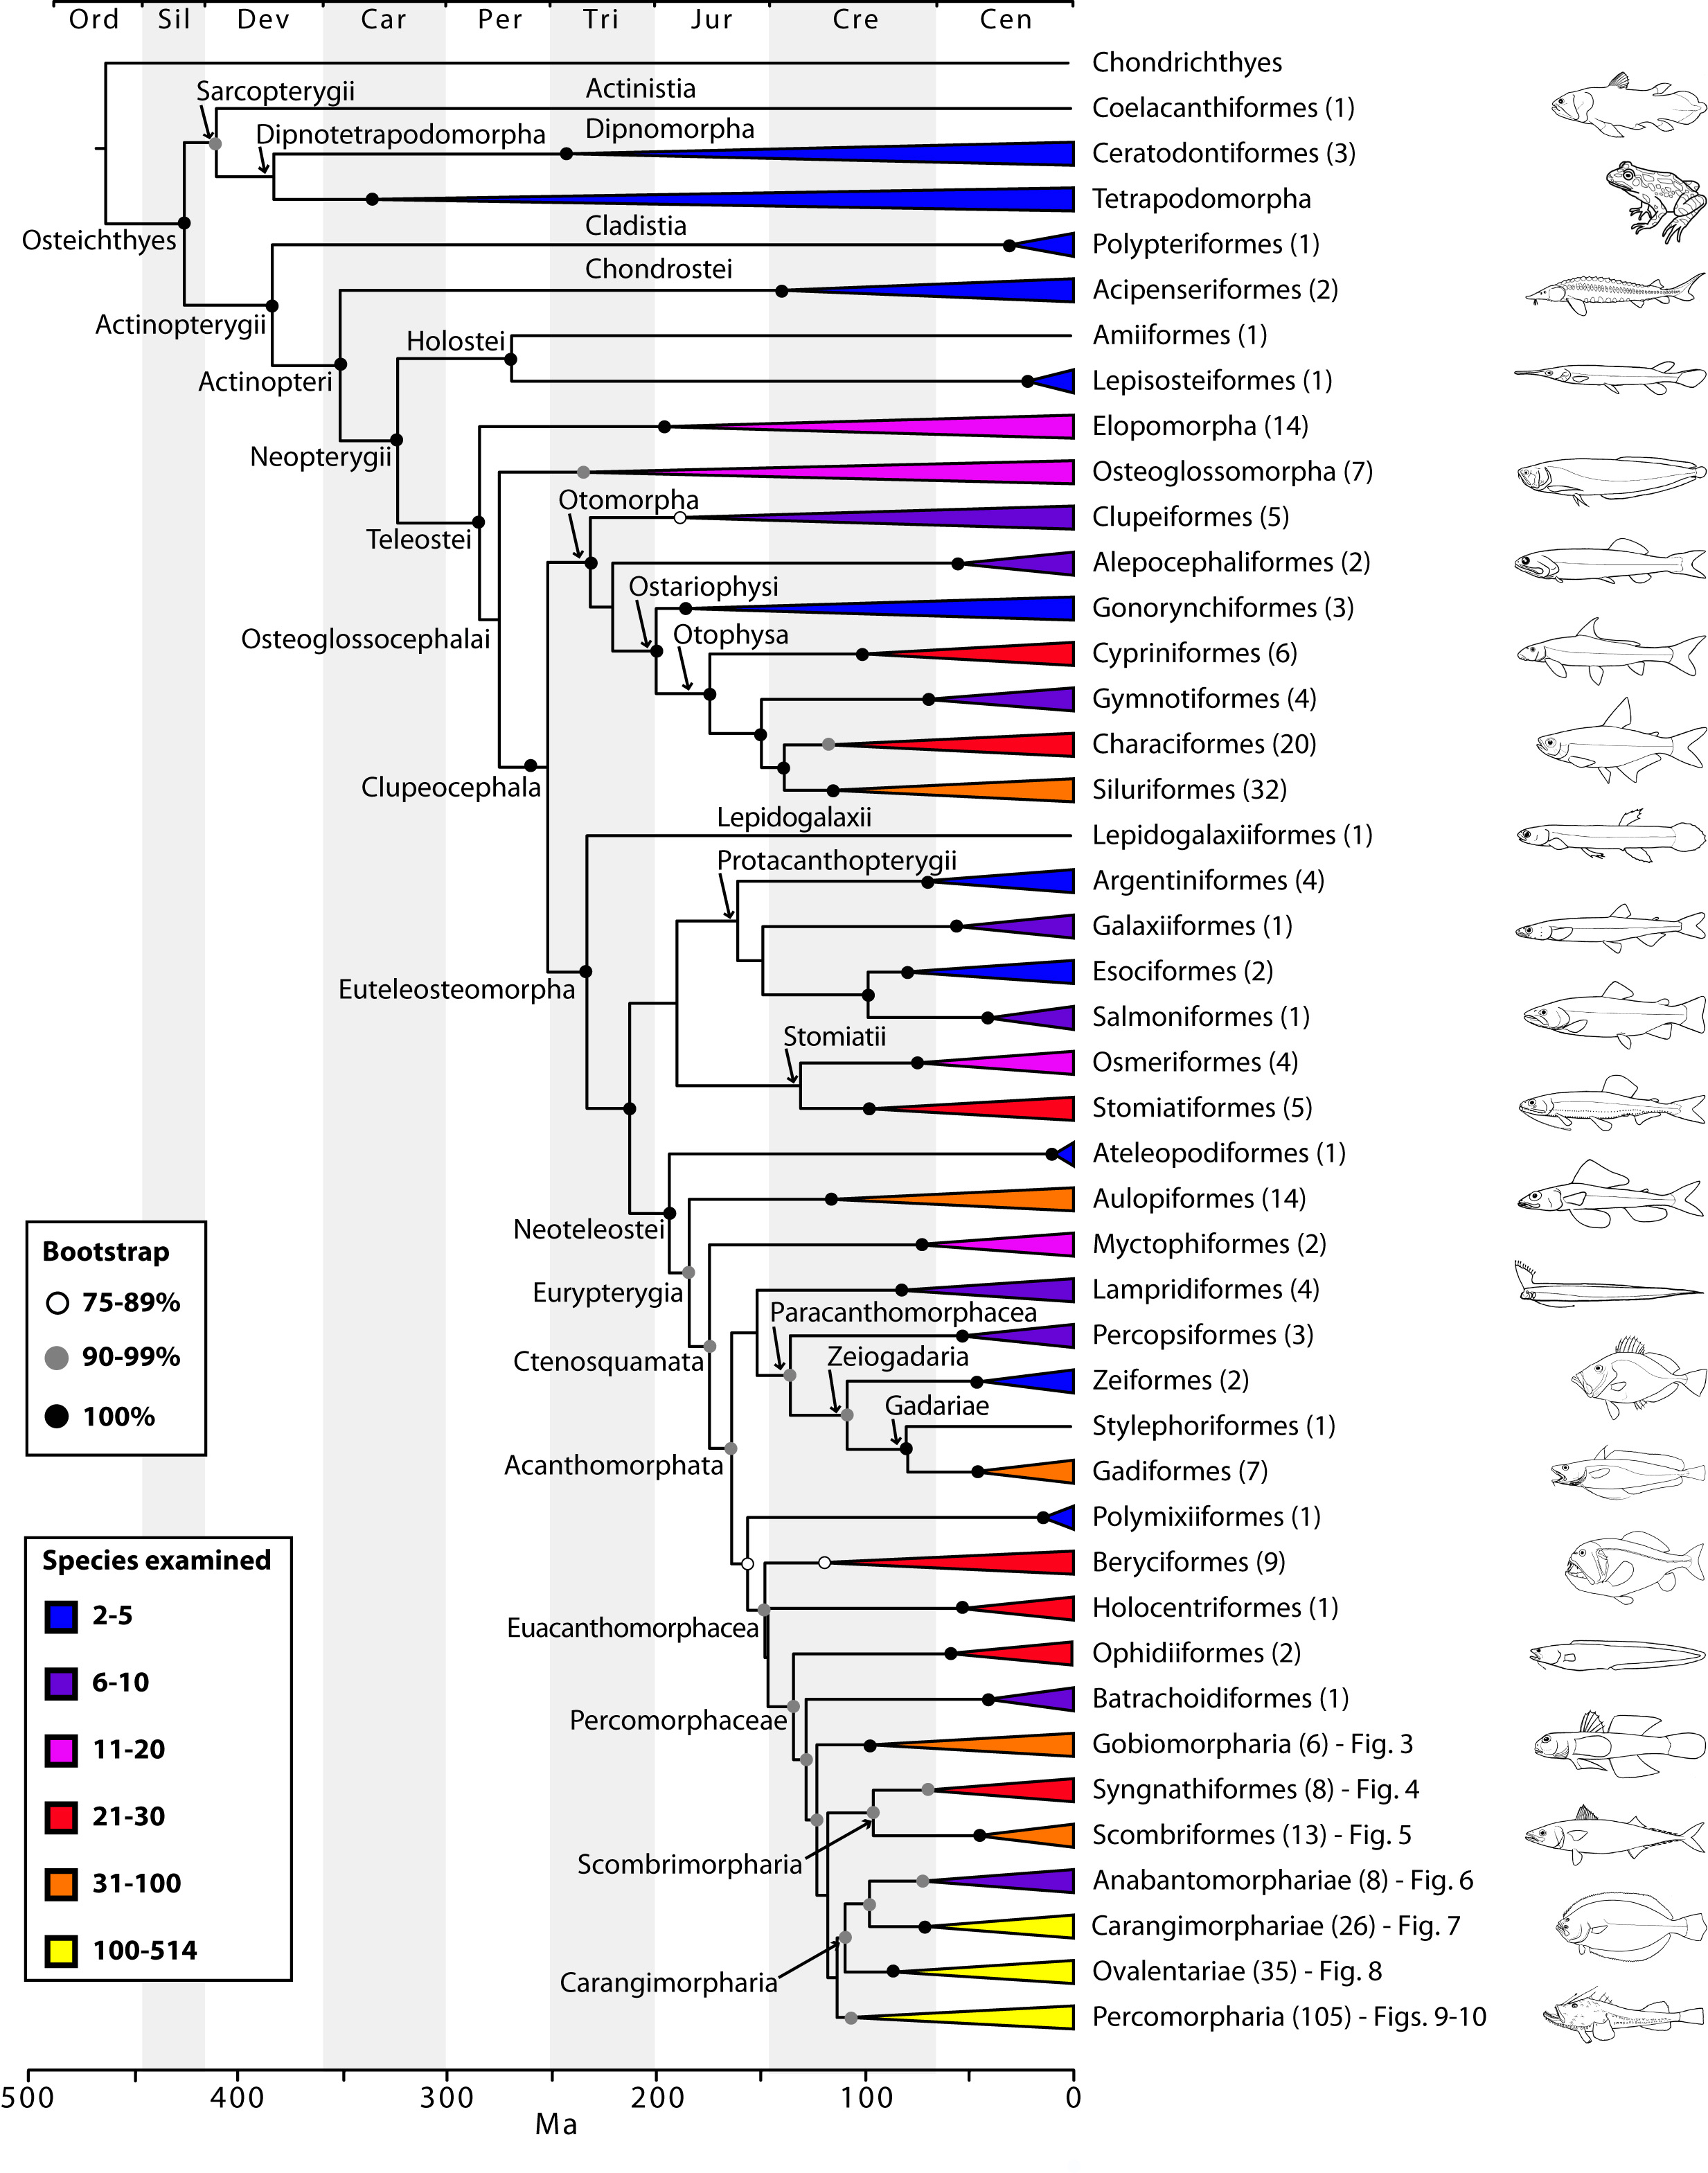
\includegraphics[width=16cm]{TreeFig.jpg}

\caption{Although not necessarily representative of the species in the dataset, this figure shows an example classification tree that TrawlExpert will build in order to allow searching of data in an intelligent way \citep{plosblog2014}.}
\label{fig:Tree}
\end{figure*}

\begin{figure*}[p]
\centering
\begin{tabular}{ p{79mm}p{79mm} }
a) & b) \\
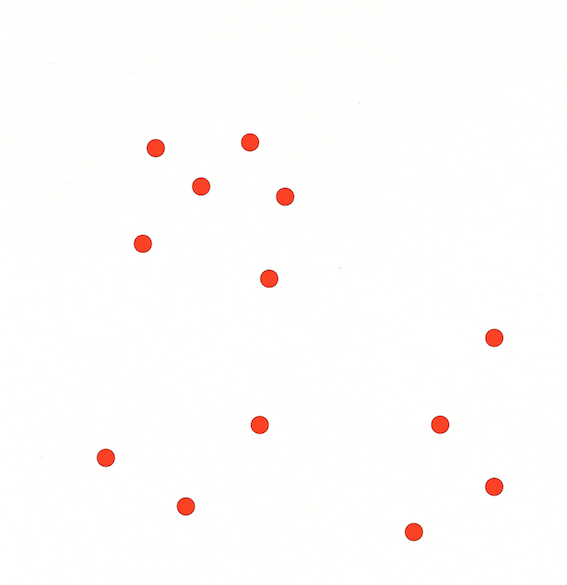
\includegraphics[width=78mm,frame=0.01cm]{Large/Fig.png} & 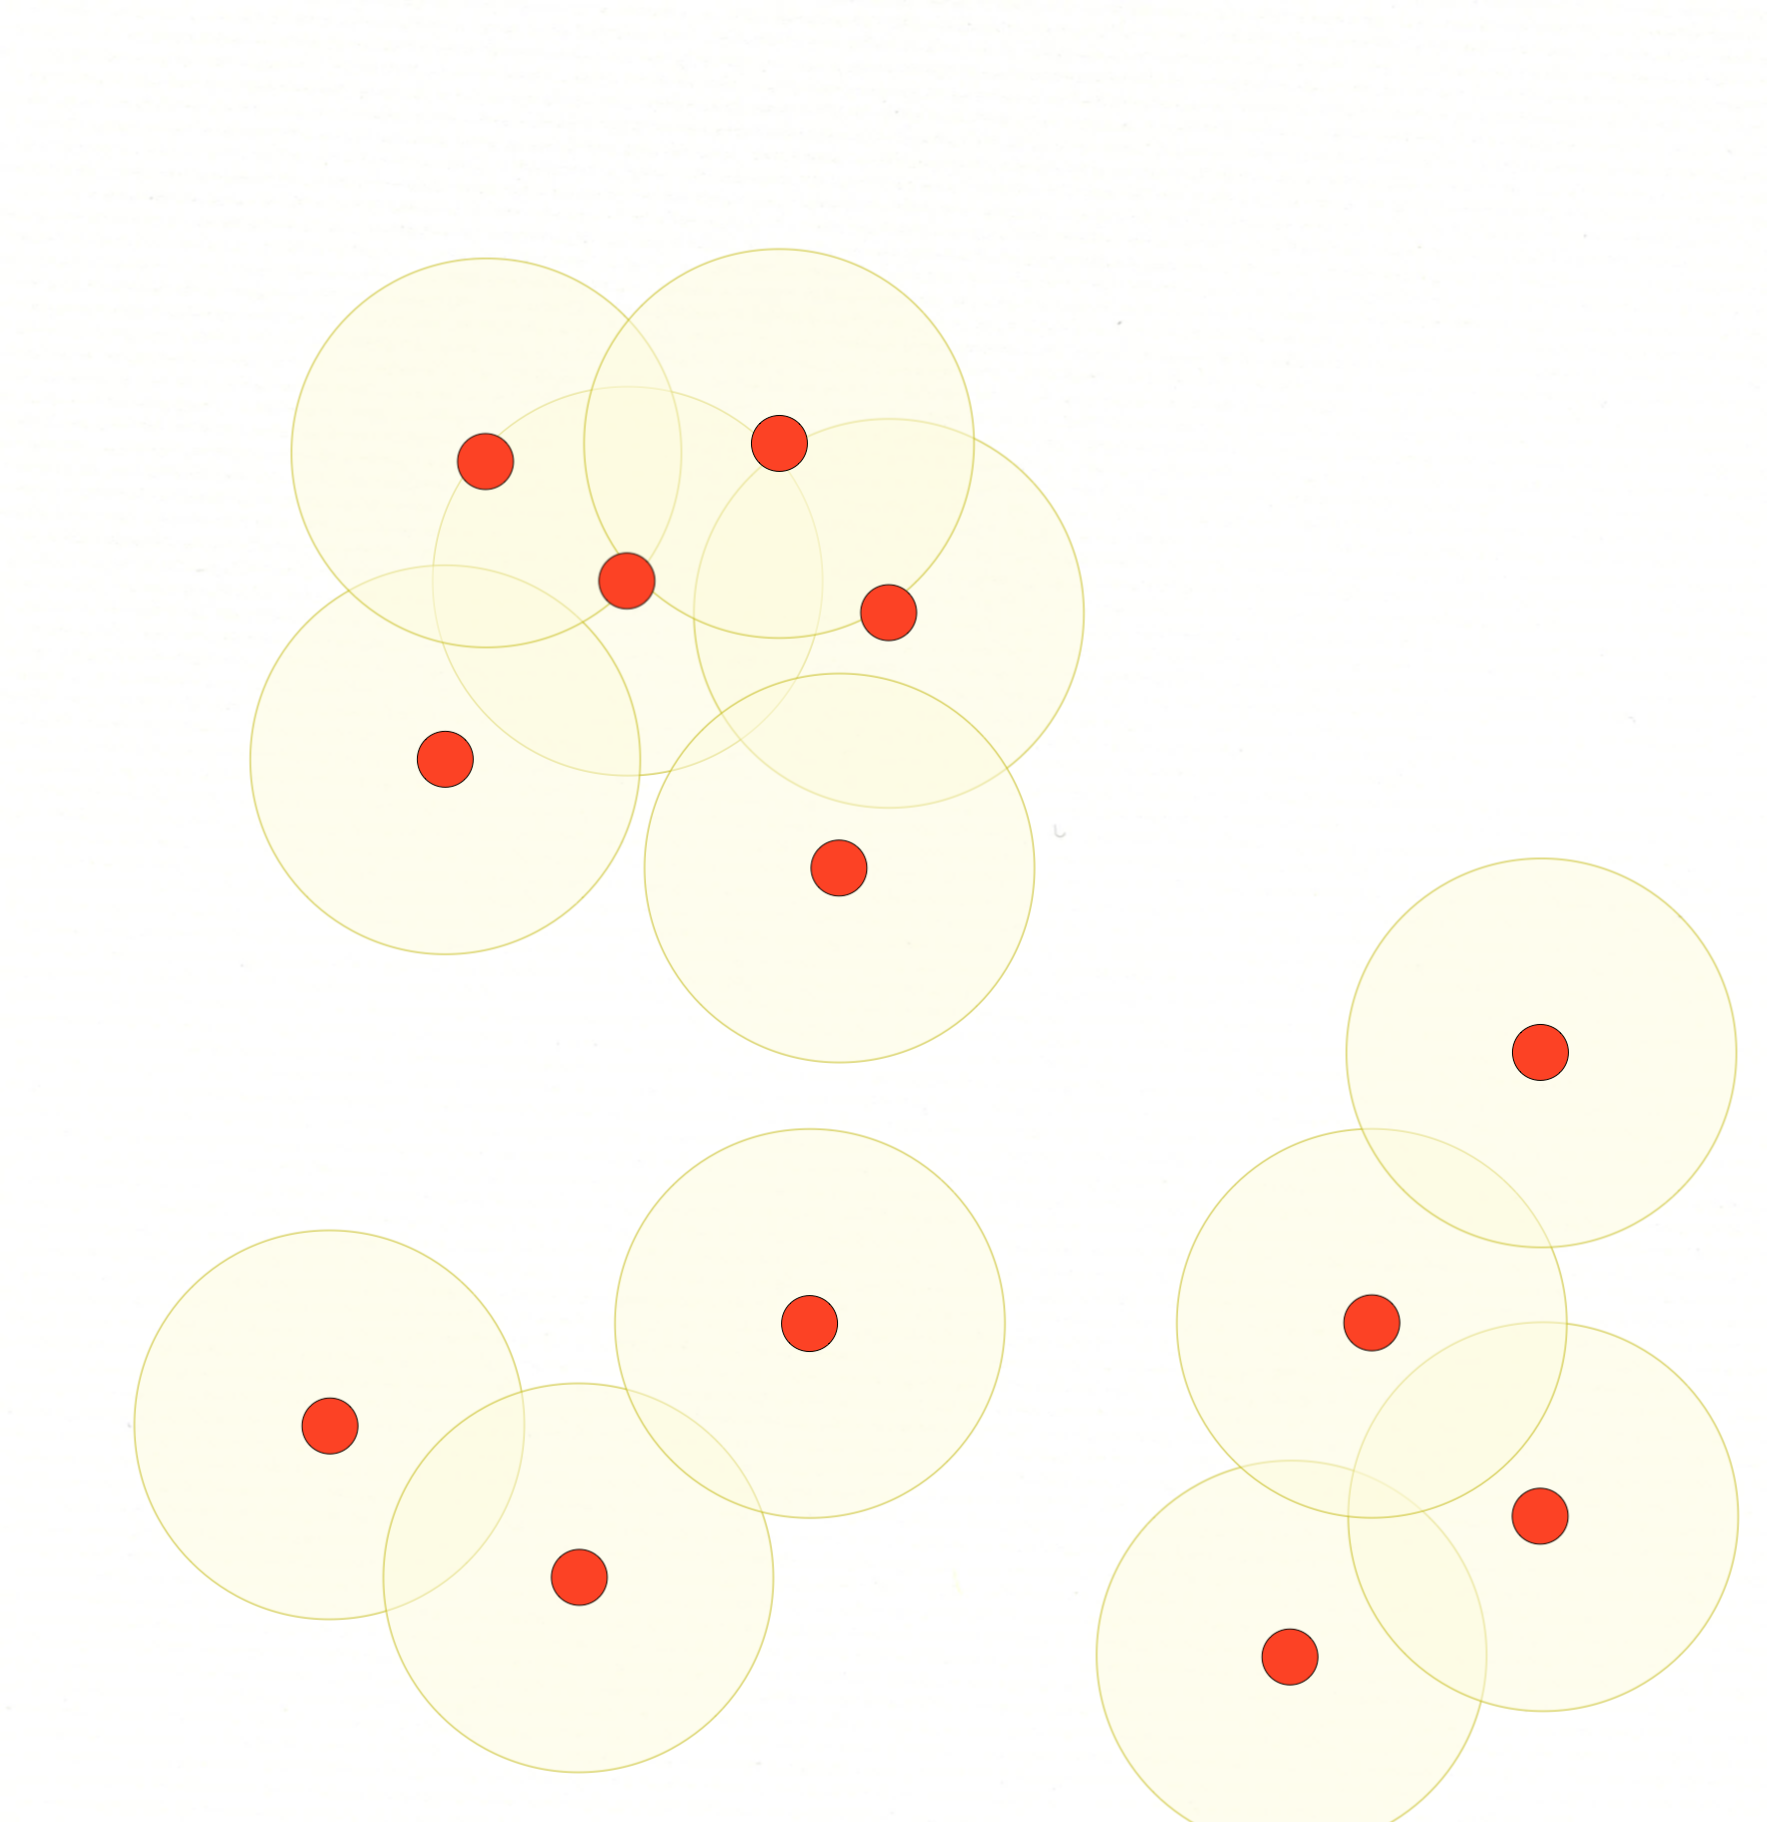
\includegraphics[width=78mm,frame=0.01cm]{Large/Fig2.png} \\
c) & d) \\
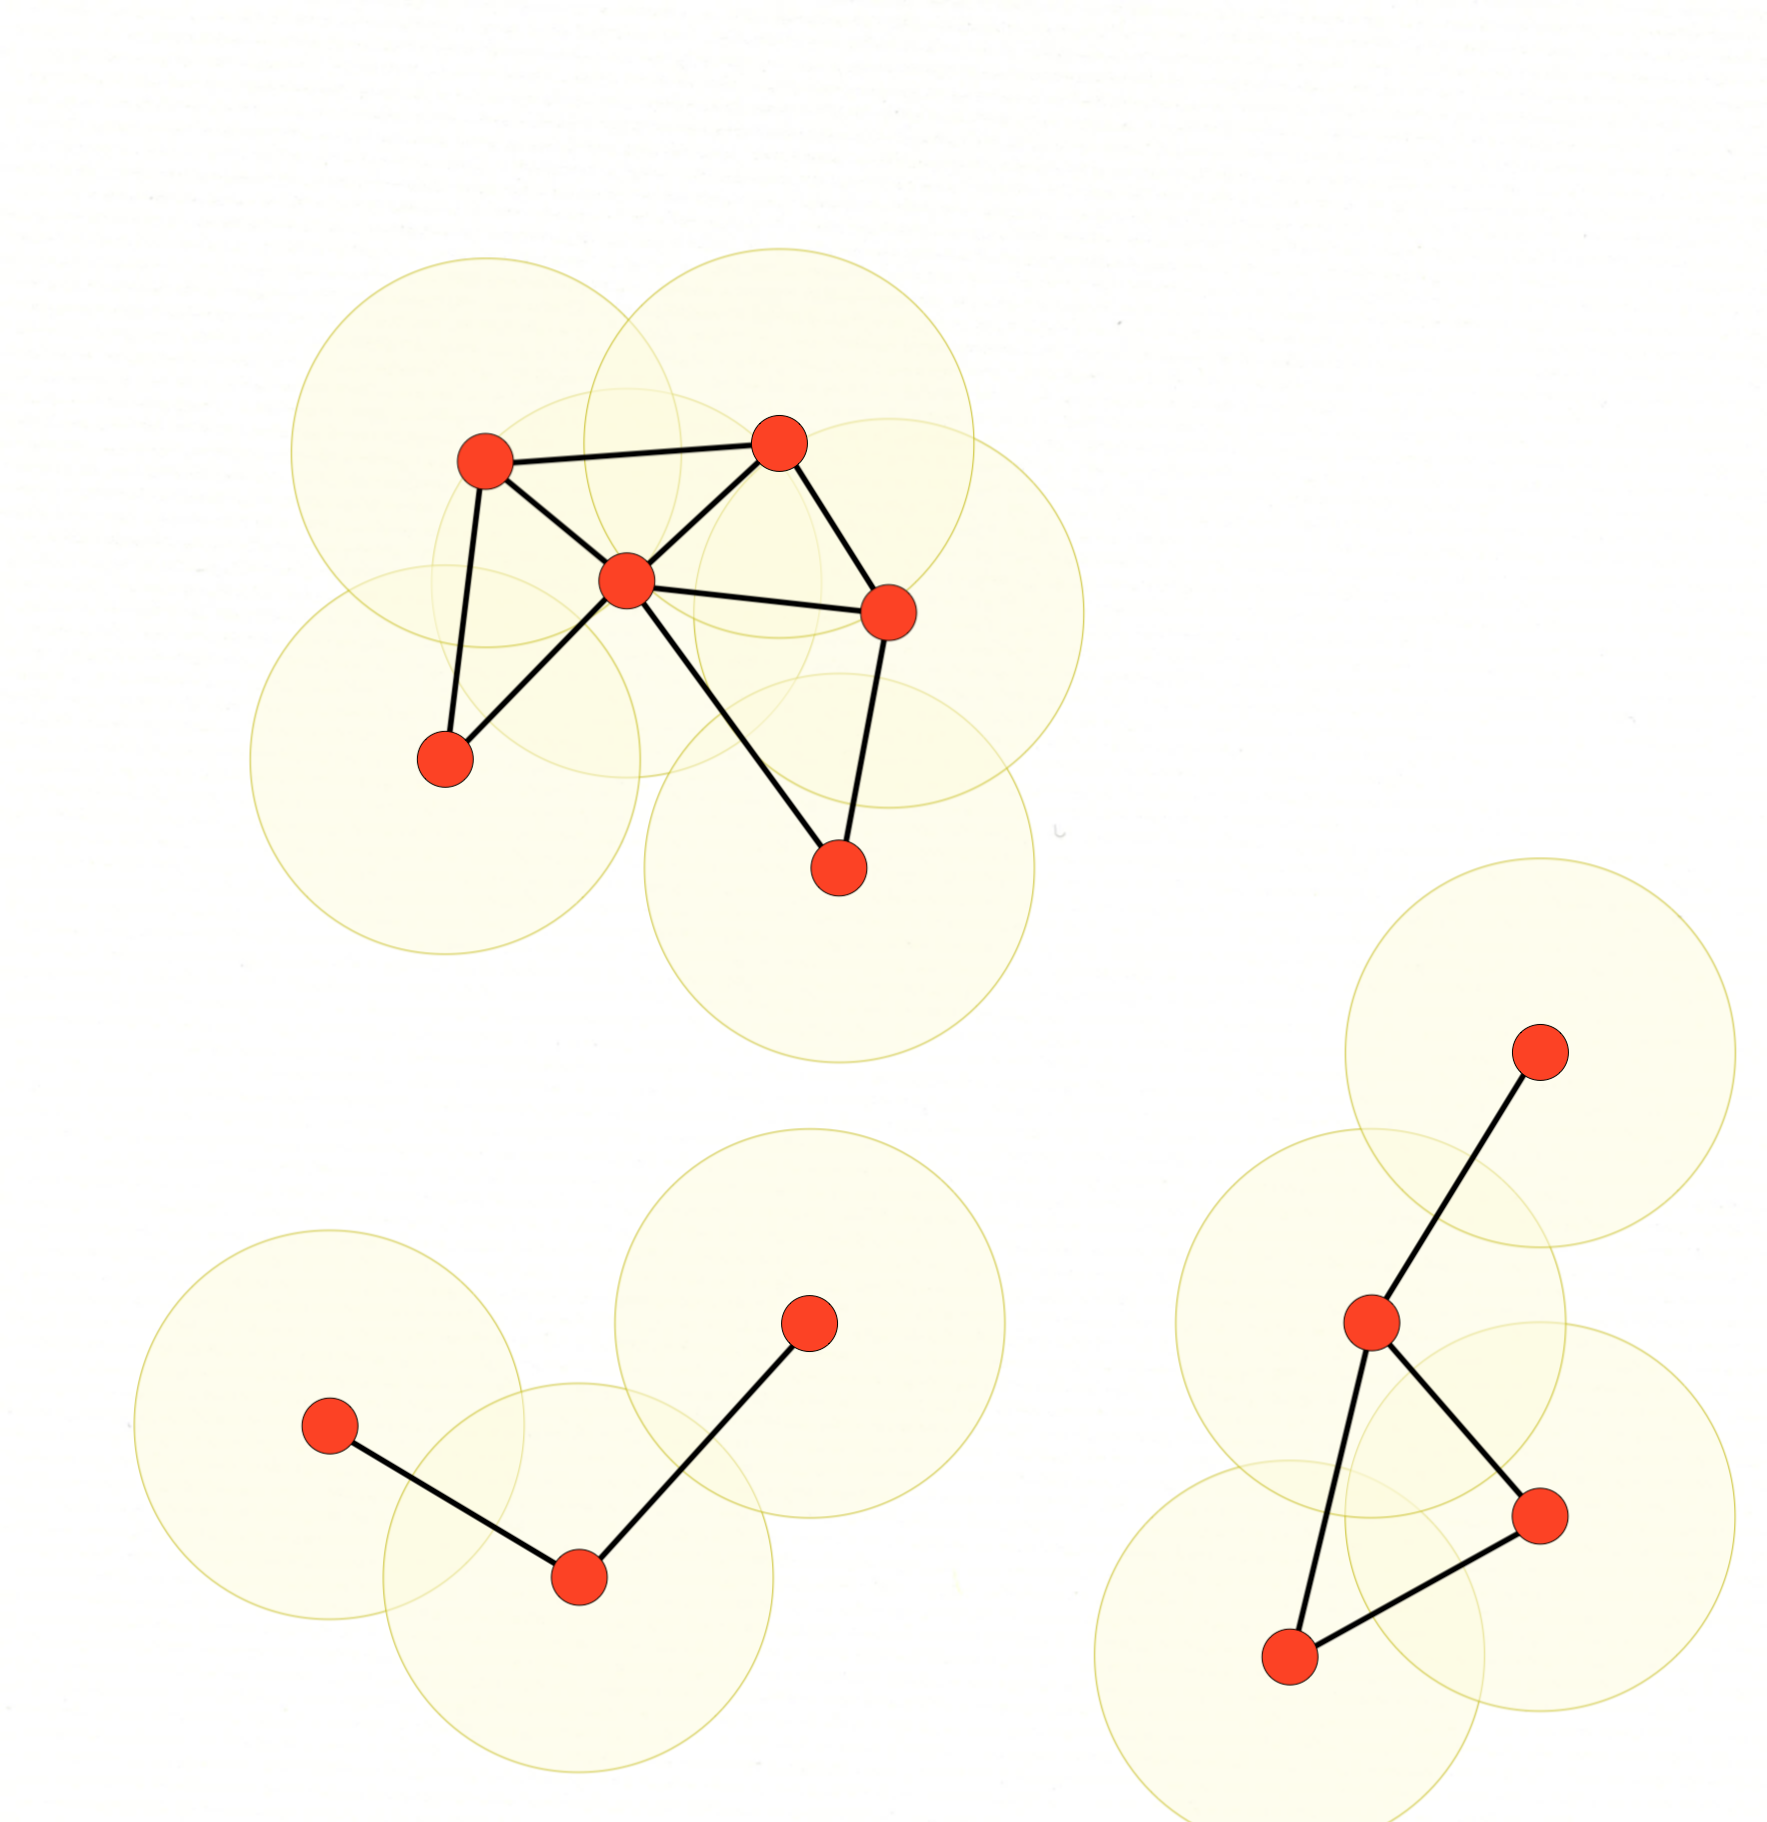
\includegraphics[width=78mm,frame=0.01cm]{Large/Fig3.png} & 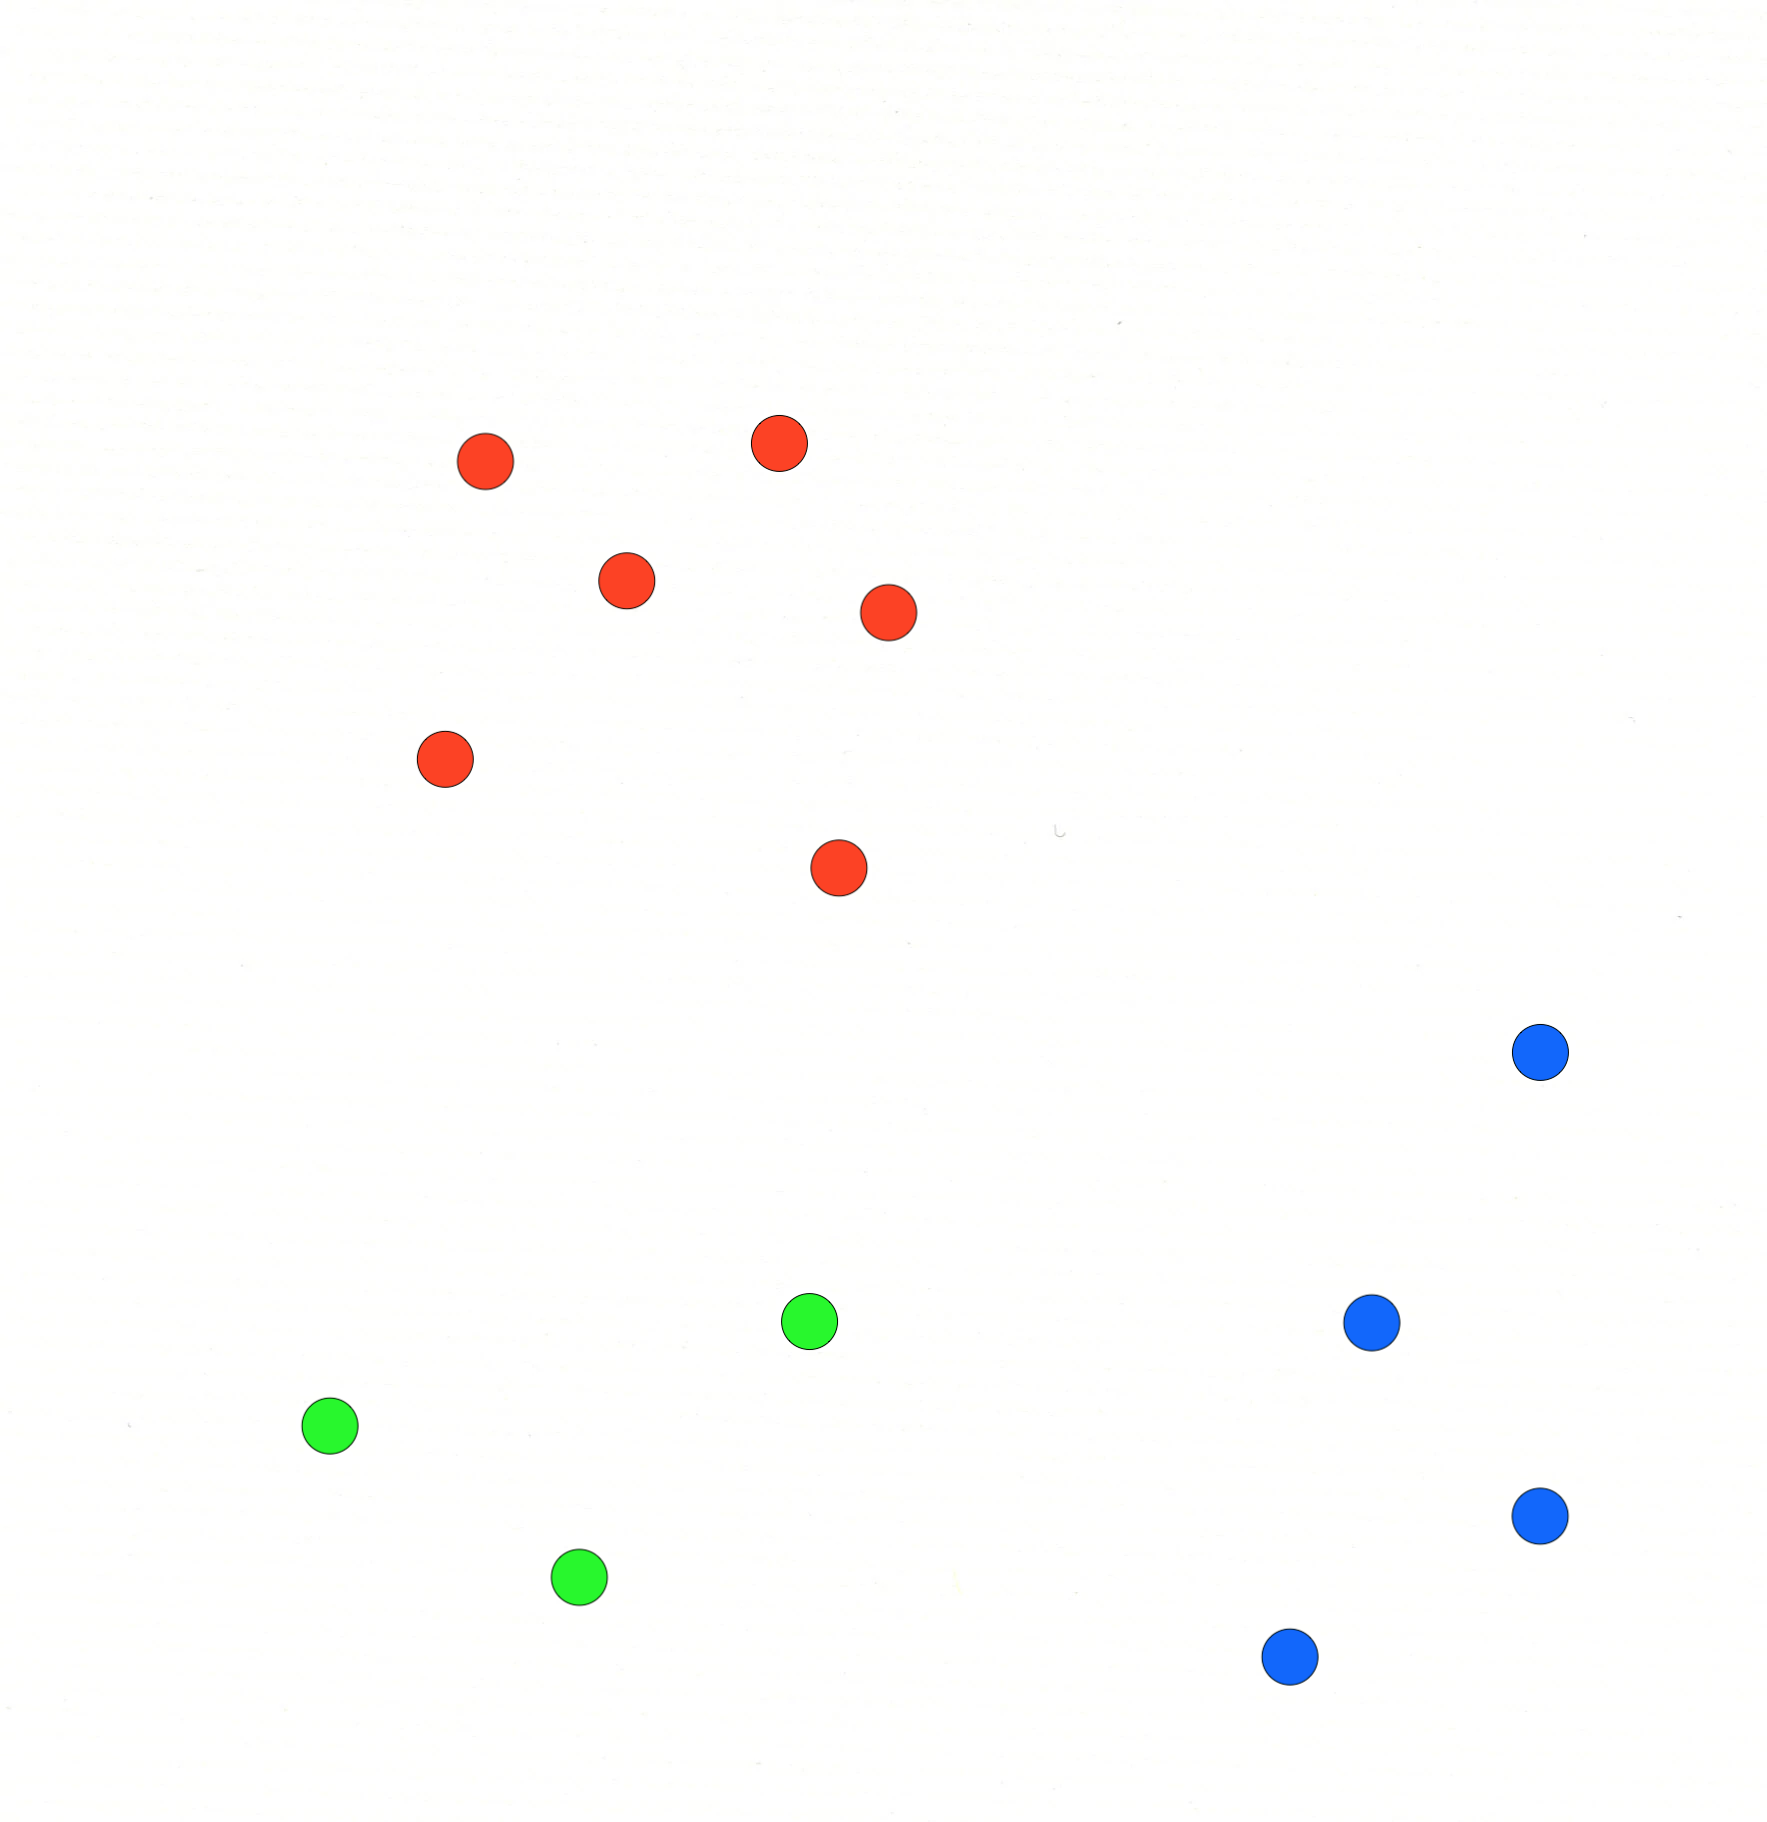
\includegraphics[width=78mm,frame=0.01cm]{Large/Fig4.png}
\end{tabular}
\caption{A visualization of the proposed algorithm for computing output 4. In a), an example search result is shown. The user wishes to classify these results into subgroups based on location. In b), a radius of similarity is chosen by the user. In c), overlapping regions determine connected nodes, creating a graph structure with groups of connected nodes. In d), the points are classified into groups by finding connected components of the graph structure using breadth-first search.}
\label{fig:Groupings}
\end{figure*}

\clearpage
\section{Project Plan}
\subsection{Milestones}
The following milestones will help inform our progress towards completing the goals. Given that the team contains 5 people, the team will be divided up into two subteams of 2-3 people for maximum efficiency. Individual members' tasks can be decided by the subteams based on the progress of that team towards completing the next milestone's goal(s). Subteams should be in constant communication and in agreement about the inputs and outputs of modules to avoid the need rewriting of code.


\begin{table}[h]
	\centering
	\begin{tabular}{p{0.16\hsize}p{0.38\hsize}p{0.38\hsize}}
		\toprule
		\textbf{Milestone} & \textbf{Subteam A} & \textbf{Subteam B}\\
		\midrule
		Milestone 1 \newline (``Bedrock'') \newline(End of Week 1)
		& Finished parsing module for .csv data to create Java objects that can be used for analysis; start data cleansing
		& General binary search module underway \\
		\midrule
		Milestone 2 \newline (``Quartz'') \newline(End of Week 2)
		& Cleansed the data to remove or correct entries not containing all of the columns; start generating biological classification tree module
		& Finished and tested binary search; start mergesort \\
		\midrule
		Milestone 3 \newline (``Granite'') \newline(End of Week 4)
		& Finished and tested biological classification tree; start formatted text output
		& Finished and tested mergesort; start writing query module for output type 1, 2 and 3 making use of the biological classification tree, mergesort and binary search to get results from data \\
		\midrule
		Milestone 4 \newline (``Sandstone'') \newline(End of Week 6)
		& Continue text output tools. Google Maps API should be explored if time allows, otherwise it can be omitted to keep the project within scope
		& Continue query module: finished output 1,  2 \& 2; start output type 4\\
		\midrule
		Milestone 5 \newline (``Diamond'') \newline(End of Week 8)
		& Finished data visualization or text output tools; prepare keynote presentation
		& Finished output type 4; prepare keynote presentation \\		
		\bottomrule
	\end{tabular}
\end{table}

\noindent While this schedule provides a good reference and a way to monitor progress, team members should be flexible and remain in communication to ensure the project is kept on schedule. For example, if a milestone is reached before its given date, the next milestone should start development early. Approximately 1-2 weeks have been purposely left as padding at the end in case of unforeseen circumstances.


\subsection{Team Roles}
\begin{table}[h]
	\centering
	\begin{tabular}{p{0.20\hsize}p{0.30\hsize}p{0.10\hsize}}
		\toprule
		\textbf{Member} & \textbf{Role} & \textbf{Subteam}\\
		\midrule
		Christoper Schankula & Team Lead & A\\		
		\midrule
		Ray Liu & TA \& Professor Liaison & A\\	
		\midrule
		Winning Liang & Project Log Admin & A\\		
		\midrule
		Haley Glavina & Meeting Minutes Admin & B\\	
		\midrule
		Lawrence Chung & Head of Booking & B\\
		\bottomrule
	\end{tabular}
\end{table}

\subsection{Workflow}

The team will use \textbf{GitLab} as the primary way of sharing code and keeping up to date. The Git repository will be split into two branches, in addition to the \textit{master} branch: \textit{TeamA} and \textit{TeamB}. Each Subteam will develop on their respective branch, then issue merge requests so the team can evaluate and approve merges into the \textit{master} branch.

\subsection{Communication}

The team will use \textbf{Slack} and \textbf{Facebook Messenger} as primary and secondary means of communication. A Slack group has been created and each of the members were invited to it. \textbf{Google Drive} will be used to keep track of documentation such as the \textit{Project Log} and meeting minutes.

\clearpage
\bibliographystyle{apa}
\bibliography{bib}


\end{document}